\documentclass[english]{uzhpub}
\usepackage[T1]{fontenc}
\usepackage[latin9]{inputenc}
\usepackage{url}
\usepackage{hyperref}
\usepackage{epstopdf}
\usepackage[round,comma]{natbib}
\interfootnotelinepenalty=10000
\bibliographystyle{abbrvnat}

\hypersetup{
    colorlinks=true,
    linkcolor=black,
    filecolor=black,      
    urlcolor=blue,
    citecolor=black
}

\renewcommand{\baselinestretch}{1.5}

\begin{document}

%% Titelei
\title{Scale-Invariant Export Contents from I/O-Tables}

%\subtitle{}

\author{Luzius Meisser, luzius@meissereconomics.com}

\date{2016-04-19}

\maketitle

%\emph{The Leontief inverse is the standard tool to calculate the import content of exports (also known as import reuse, foreign contents of exports, foreign value added and vertical specialization) from given input-output tables. Unfortunately, it only yields correct results when the inputs are proportionally used for the production of the outputs in each sector, which rarely is the case. As a consequence, input reuse as calculated by the Leontief inverse depends on the resolution of the underlying data. In case of the WIOD dataset, global average import reuse climbs steadily from 17\% to 25\% as the resolution is increased from one to thirty-five sectors per country. I address this known problem by postulating a hidden variable 'propensity for processing trade' for each country to construct a scale-invariant computation method, resulting in a more credible -- but probably still too low -- value of 32\% globally.}

\emph{The Leontief inverse is the standard tool to calculate the import content of exports from given input-output tables. Unfortunately, it only yields correct results when inputs are proportionally used for the production of outputs, which rarely is the case. As a consequence, the value calculated by the Leontief inverse depends on the resolution of the underlying data. With the WIOD dataset, global import contents of exports climb from 17\% to 25\% as the resolution is increased from one to thirty-five sectors per country. I address this known problem by constructing a new, scale-invariant computation method, resulting in more credible 32\%.}

\section{Introduction}
% The OECD refers to import reuse as \href{http://www.oecd-ilibrary.org/trade/data/oecd-wto-statistics-on-trade-in-value-added_data-00648-en}{foreign value added share of gross exports}  Sometimes, the term "import contents of exports" (e.g. http://www.wiod.org/publications/papers/wiod5.pdf), but not consistently across different sources (OECD differs).
Import reuse is a basic metric that is typically derived from input-output tables and often serves as an intermediate step for more elaborate calculations, for example for estimating exchange-rate pass-through. \citep{auer2016international} Import reuse measures the extent to which exports consist of previous imports and is sometimes also referred to as import content of exports, foreign contents of exports, foreign value added share of gross exports, or foreign value added; whereas the exact definition can vary. \cite{hummels2001nature} interpret it as \emph{vertical integration}. Its usual method of calculation is to derive the composition of exports by applying the Leontief inverse to a national input-output table.

The known problem with the traditional approach is that the Leontief inverse implicitly assumes proportional use of inputs. In practice, however, firms that import much also tend to export much, resulting in a large share of processing trade. \citep{amiti2012importers} When firms that engage heavily in processing trade are aggregated with firms whose activities are mainly domestic, information about the actual use of specific imports gets lost and the import reuse as calculated by the Leontief inverse decreases. As a result, the Leontief inverse systematically underestimates import reuse for most countries. According to \cite{oecd2000}, Mark Planting was the first to observe this effect in 1991 when comparing the import reuse derived from a dataset with a resolution of 6800 sectors versus a dataset with 536 sectors. That is why the OECD considers the Leontief result a "conservative indicator of the actual input activity".

\cite{koopman2012estimating} as well as \cite{kee2013domestic}, both focusing on China, address this problem by enriching input-output tables with additional data to isolate processing trade. Koopman et al. summarize their approach as follows: "The basic idea is to use information from the standard I/O table to determine sector-level total imports/exports, and information from trade statistics to determine the relative proportion of processing and normal exports within each sector." Similarly to the findings presented in here, they find that actual import reuse is much higher than what the traditional approach suggests. Generally, it would be desirable to have a method that provides plausible results without requiring tedious amounts of detailed trade data that in practice is often hard to obtain. And that is exactly what I present: a method to better estimate import reuse from input-output tables alone, under the assumption of self-similarity.

Generally, I view trade flows as a graph and not as a matrix, a choice motivated in section \ref{sec:data}, which also describes the used data more closely. Section \ref{sec:method} specifies the applied methods, in particular how introducing a hidden variable \emph{processing trade propensity} allows the calculated import reuse to be tuned such that it becomes robust against changes in resolution (scale-invariance). This is followed by results section \ref{sec:result}, that presents selected findings, and a concluding section \ref{sec:conclusion}. All source code, input data, and outputs can be found on \href{http://importreuse.meissereconomics.com}{importreuse.meissereconomics.com}.

\section{Data} \label{sec:data}
\subsection{World Input-Output Database}
The world input-output database (WIOD) presented by \cite{timmer2012world} serves as data source. It covers 40 countries and 17 years starting from 1995 with a resolution of 35 actual sectors per country plus five sectors for different forms of final use. It differs in three ways from other input-output tables, all of which lead to lower calculated values of import reuse, making direct comparisons to results based on other datasets difficult.

First, WIOD contains disaggregate flows between individual sectors across countries. This allows to better account for trade flows that go back and forth between countries and thereby better identifying returning exports, i.e. imports into a country that originally stem from the country itself. Accounting for this effect, calculated import reuse can decrease by a few percent. Second, WIOD unfortunately does not include obvious re-exports (see section 4.2 of \cite{dietzenbacher2013construction}), which is a form of processing trade and something I would have preferred to capture. Third, WIOD allows imports to directly flow into domestic final use, which is more realistic than other input-output tables that require all imports to first flow through a domestic sector before they can be consumed. The imports that directly flow into final use have no chance of being re-exported, so this again leads to a lower calculated import reuse than with other data sources.

An advantage of using WIOD is that unlike other input-output tables, it does not contain an "other" sector, which is typically used to collect all trade flows that are hard to assign to other sectors. For example, the "other" sector of the US input/output tables provided by the Bureau of Economic Analysis\footnote{\href{http://www.bea.gov/industry/io_annual.htm}{www.bea.gov/industry/io\_annual.htm}} predominantly consists of unrelated imports and exports, creating the illusion of a sector with large amounts of processing trade and distorting import reuse upwards by multiple percentage points.

Each sector has a hidden implied input I call \emph{value creation}, which is simply defined as the sum of all outputs minus the sum of all other inputs. It represents the value added in that sector. For simplicity, I merge the five final use sectors of each country into a single consumption node that is treated specially and not counted as a sector. I.e., when later reducing the number of sectors per country to one, there will actually be two nodes left per country, one actual sector and the consumption node. Furthermore, I ignore negative flows into final use\footnote{This can happen when capital is reduced or inventories decrease.} as they are negligible and not having negative edge weights is a prerequisite for the Edmonds-Karp algorithm used later. \citep{edmonds1972theoretical} All other flows in WIOD are already zero or positive.

\subsection{Graph View}
\label{sec:graphview}
Usually, economists treat input-output tables as matrices. An equally valid and in this case more insightful view is to treat input-output tables as weighted directed graphs. Every square matrix can be represented as a weighted directed graph and a weighted directed graph can converted into a square matrix as long as there is at most one edge in each direction between each pair of nodes. In the graph representation of input-output tables, each node represents a sector in a country and is named accordingly. Each weighted edge $e=(a, b, w)$ represents a flow from node $a$ to node $b$ of volume or weight $w$. Flows from a node to itself are allowed and correspond to diagonal elements in the matrix view.

When merging two nodes $a$ and $b$ of a graph into a new node $c$, the nodes $a$ and $b$ are replaced by $c$ in all edges and then all edges that connect the same nodes in the same direction aggregated into a single new edge whose weight is the sum of the old weights. This is equivalent to first removing column $i$ and adding it to column $j$, and then also removing row $i$ and adding it to row $j$ in the matrix view, with $i$ and $j$ being the indices of the two sectors represented by nodes $a$ and $b$. When doing so, the indices of other sectors may change, making it less convenient to track a specific sector in the matrix view than in the graph view, where the names of unaffected nodes stay the same. Generally, the graph view is more compact than the matrix view when the matrix is sparse and enables a more intuitive representation of the trade flows.

\section{Method}
\label{sec:method}

\subsection{Varying the Sector Resolution}
\label{Varying}
The usual method to calculate input reuse is to apply the Leontief inverse to the input-output table. A known flaw of this approach is that it implicitly assumes proportional use of inputs.\footnote{For the avoidance of doubt, this is \emph{not} what is usually called the proportionality assumption. The proportionality assumption in the context of input-output analysis refers to proportionally assigning an import to domestic sectors. In contrast, proportional use of inputs refers to proportionally assigning the inputs (including domestic value creation) of a single sector to its outputs (including consumption).} This is no problem for disaggregate data with atomic resolution, but when applied to aggregate data, the Leontief inverse is systematically biased in the presence of processing trade. The import reuse calculated by the Leontief inverse usually grows as the resolution of the underlying data is increased. In case of the WIOD data, world input reuse grows from 17\% to 25\% as the resolution is varied between one and thirty-five sectors (see section \ref{res:varying}), illustrating that the Leontief inverse is not scale-invariant. A scale-invariant computation method that is consistent across different resolutions would yield more credible results, which is what will be constructed in the subsequent sections.

\subsection{Maximum Flow}
Given the input-output graph of a country, one can derive the minimum and maximum possible import reuse by computing the maximum amount of imports that can flow into domestic consumption (for the minimum) or into exports (for the maximum). The true import reuse must lay somewhere in between. This is known as the \emph{maximum flow problem} and can for example be solved with the Edmonds-Karp algorithm. \citep{edmonds1972theoretical} Unfortunately, the calculated bounds usually turn out to be so wide that they provide only little guidance as to where the true import reuse might be.

\subsection{Processing Trade Propensity}
To seek plausible values of import reuse within the given bounds, I introduce a parameter \emph{processing trade propensity} $s_{proc,c} \in [0,1]$ for each country $c$. It is defined as the share of inputs (excluding value creation) of a node that are directly assigned to its outputs (excluding domestic consumption). Afterwards, the remaining inputs are proportionally assigned as before. This is equivalent to splitting the node in two, namely a processing node and a normal node as illustrated in figure \ref{fig:sketch}.

\begin{figure}
\centering
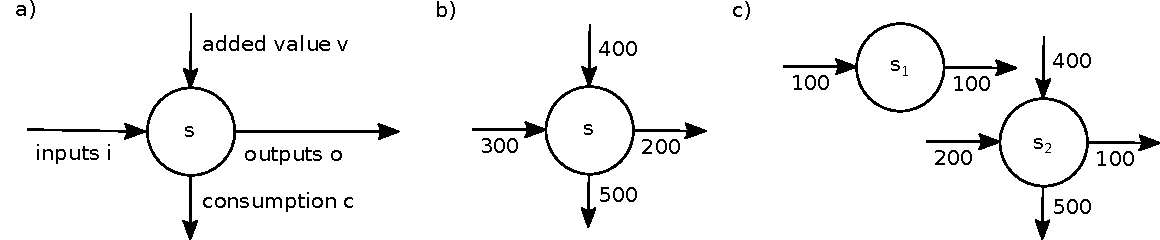
\includegraphics[scale=0.8]{../results/sketch}
\caption{In order to separate processing trade, the flows of a sector $a$ are divided into four groups. There is the sum of all inputs $i$, flows towards domestic consumption $c$, and the sum of all other outputs $o$, thereby implicitely providing the added value $v = c + o - i$. Given a processing trade propensity $s_{proc}$, the sector $s$ is split into two new nodes, with $s1$ only having horizontal processing flows of magnitude $i_{s1}=o_{s1}=min(i, o, s_{proc} \frac{i+o}{2})$, here with $s_{proc}=0.4$. In figure b, the Leontief inverse would suggest that $3/7=43\%$ of the outputs stem from prior inputs. After the split in figure c, this number increases to $\frac{1/1 + 2/6}{2}=67\%$.}\label{fig:sketch}
\end{figure}

By exogenously varying $s_{proc}$, an interval of potential true values of import reuse can be explored, with $s_{proc}=0$ corresponding to the proportional use of inputs as implicitely assumed by the Leontief inverse, and $s_{proc}=1$ being somewhere between the proportional result and the maximum flow result. Even though $s_{proc}=1$ does not reach the maximum flow result, it seems to suffice for our purpose.\footnote{Generally, maximum flow can only be reached by redirecting locally created value over multiple nodes towards consumption. The Edmongs-Karp algorithm does this, but my method does not as it is strictly based on locally available information.} In the data at hand, the only country that would have a slightly negative processing trade propensity for some of the given years is Russia, so imposing $s_{proc}\geq0$ is unproblematic.

\subsection{Scale-Invariance}
\label{met:scale-invariance}
Equipped with a parameter to tune, one can try to find values of $s_{proc}$ that make the calculated import reuse scale-invariant. One can do this globally with one global $s_{proc}$, or nationally with a separate processing trade propensity $s_{proc, c}$ for each country $c$. In both cases, the parameter is adjusted such that the covariance $cov(r, f)$ of resolution $r$ (the number of sectors per country) and resulting import reuse $f$ is minimized. I calculate import reuse iteratively by repeatedly updating the composition of inputs for each node in the worldwide input-output graph until the values stabilize. On a higher level, binary search is used to find the $s_{proc, c}$ that minimizes $cov(r, f_c)$ for each country $c$.

Being robust against changes in resolution, the import reuse resulting from assuming the scale-invariant processing trade propensity is more plausible than the one calculated with proportional use of inputs. Under the assumption that it is also robust against further changes in resolution beyond the limits of the data at hand, the calculated scale-invariant import reuse matches the true import reuse. This assumption is valid if the input-output graph is self-similar, i.e. if the relevant properties of the network stay the same at all scales. This bold assumption is qualitatively supported by \cite{song2005self}, who observed that a wide range of real-world networks exhibit self-similarity. Furthermore, \cite{chaney2014network} uncovers dynamics in international trade that resemble the algorithm proposed by \cite{barabasi1999emergence} to construct scale-free, self-similar networks. Also, the node connectivities of a scale-free network follow a power-law distribution, which is ubiquituous in economics according to \cite{gabaix2016power}. Thus, the assumption of self-similarity is not far-fetched and probably even is the most natural assumption one can take in absence of evidence to the contrary.

\section{Result}
\label{sec:result}

\subsection{Varying the Resolution}
\label{res:varying}

Figure \ref{fig:varying} shows how the average global import reuse depends on the resolution of the underlying data when it is calculated with the traditional method of applying the Leontief inverse. As the number of sectors is increased from one to the thirty-five, import reuse climbs from 17\% to 25\%. This is a clear signal that the true global import reuse is higher still.

\begin{figure}
\centering
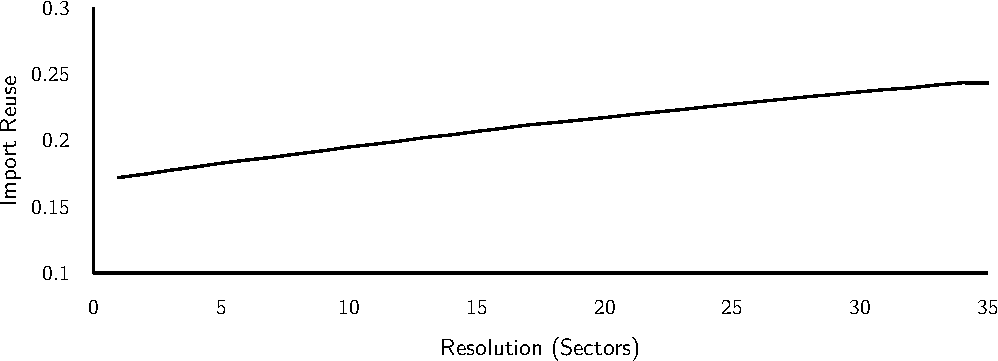
\includegraphics[scale=0.8]{../results/resolution}
\caption{The average global import reuse as calculated by the Leontief inverse grows from 17\% to 25\% as the resolution is increased from one to thirty-five sectors (2011 data, average result of 100 randomized runs).} \label{fig:varying}
\end{figure}

The program to calculate the data behind figure \ref{fig:varying} first parses the given world input-output table into a graph, and then repeats calculating import reuse and reducing the number of sectors in each country by one until there is only one left. This is done by randomly selecting two sectors in each country and merging them as defined in section \ref{sec:graphview}. The reported import reuse is a global volume-weighted average across all countries. Each country's import reuse is calculated by repeatedly updating the input composition of each node until all values have converged towards a stable global equilibrium. This latter step is equivalent to applying the Leontief inverse to the matrix view. When plotting the same curve for the 40 available countries individually, results vary, but all except Russia's import reuse raise as the resolution increases. For Russia, the curve slightly declines, at least for some of the years in the dataset, indicating that the processing trade propensity of Russia is slightly negative.

\subsection{Tuning Processing Trade Propensity}
As a next step, processing trade propensity $s_{proc}$ is varied as described in section \ref{met:scale-invariance}. Figure \ref{fig:globalpref} shows how the slope of the previously shown curve changes as $s_{proc}$ is increased from $0.0$ (equivalent to the Leontief approach) to $1.0$ in steps of $0.1$, in this case for Germany in 2011. For $s_{proc}=0.686$, calculated import reuse is quite flat, with a covariance between resolution and import reuse of $cov(r, f) = 1.5x10^{-6}$, and variance $var(f)=1.9x10^{-6}$. For other countries, variances between $10^{-7}$ and $10^{-4}$ are found. Depending on the country and the year, the scale-invariant value of $s_{proc}$ varies. Figure \ref{fig:reusedrivers-processing-trade-greece} shows how processing trade propensity, scale-invariant import reuse, and Leontief import reuse change over time for Greece, a country with a more interesting development over time than others. Table \ref{tab:ranking} ranks countries by processing trade propensity for 2011. The full dataset of all countries and all years is available from the repository as \href{https://github.com/meisserecon/importreuse/blob/master/results/all.csv}{results/all.csv}.

\begin{figure}
\centering
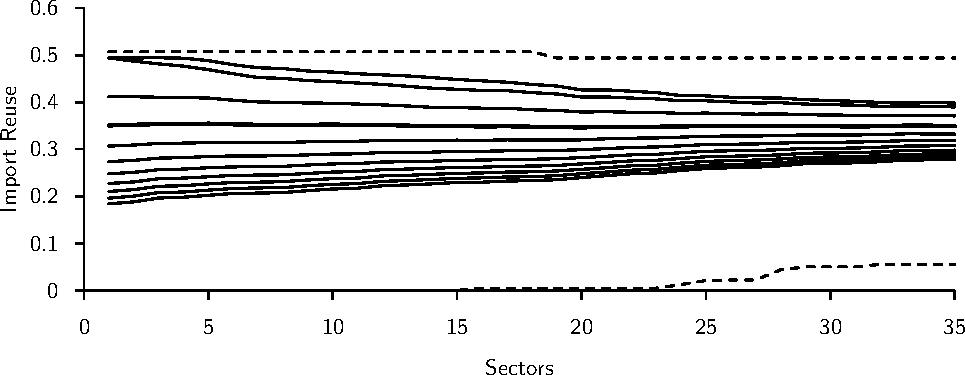
\includegraphics[scale=0.8]{../results/germanrelief2011}
\caption{Increasing processing trade propensity from $0.0$ to $1.0$ in steps of $0.1$ results in 11 curves with varying slope, all converging towards the true import reuse. If the input-output graph is self-similar, a flat curve will stay flat. If not, the curves could in principle turn towards any value within the bounds (dotted lines, less smooth because not averaged over multiple runs). The curves shown here are for Germany in 2011, suggesting a true import reuse of 35\% instead of the 28\% calculated with the traditional method (lowest continuous line).} \label{fig:globalpref}
\end{figure}

\begin{figure}
\centering
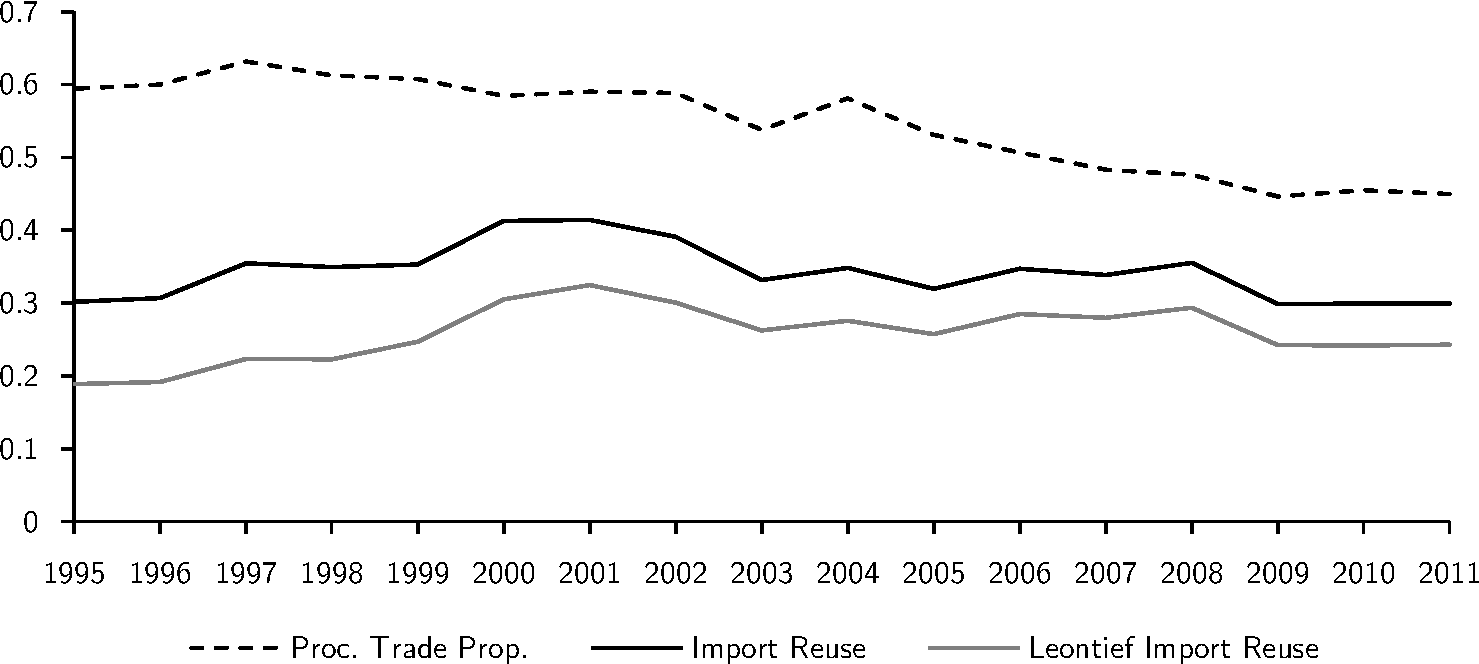
\includegraphics[scale=0.6]{../results/reusedrivers-processing-trade-greece}
\caption{Historic changes of processing trade propensity, scale-invariant import reuse, and Leontief import reuse of Greece. Greece was chosen for having a more dynamic history than other countries in the dataset.} \label{fig:reusedrivers-processing-trade-greece}
\end{figure}


\renewcommand{\baselinestretch}{1.0}

\begin{table}[]
\centering
\begin{tabular}{llll}
\textbf{Country}        & \textbf{Proc. Trade Prop.} & \textbf{Import Reuse} & \textbf{Leontief Result} \\
Czeck Republic & 0.78                        & 0.55                  & 0.46           \\
Slovakia       & 0.77                        & 0.52                  & 0.42           \\
Poland         & 0.77                        & 0.48                  & 0.34           \\
Belgium        & 0.76                        & 0.54                  & 0.46           \\
France         & 0.76                        & 0.39                  & 0.29           \\
Spain          & 0.75                        & 0.40                  & 0.30           \\
Luxemburg      & 0.74                        & 0.64                  & 0.61           \\
Taiwan         & 0.74                        & 0.51                  & 0.47           \\
Sweden         & 0.73                        & 0.41                  & 0.32           \\
Hungary        & 0.73                        & 0.55                  & 0.46           \\
Austria        & 0.73                        & 0.44                  & 0.34           \\
Netherlands    & 0.72                        & 0.47                  & 0.39           \\
Italy          & 0.72                        & 0.37                  & 0.27           \\
Japan          & 0.71                        & 0.24                  & 0.17           \\
Korea          & 0.71                        & 0.46                  & 0.40           \\
Slovenia       & 0.71                        & 0.44                  & 0.36           \\
Denmark        & 0.70                        & 0.43                  & 0.37           \\
Portugal       & 0.69                        & 0.39                  & 0.28           \\
Germany        & 0.69                        & 0.34                  & 0.27           \\
Bulgaria       & 0.69                        & 0.44                  & 0.35           \\
India          & 0.69                        & 0.30                  & 0.22           \\
China          & 0.68                        & 0.26                  & 0.22           \\
Finland        & 0.67                        & 0.41                  & 0.34           \\
Turkey         & 0.66                        & 0.31                  & 0.22           \\
United Stats   & 0.65                        & 0.21                  & 0.15           \\
Malta          & 0.64                        & 0.47                  & 0.39           \\
Mexico         & 0.64                        & 0.36                  & 0.30           \\
Estonia        & 0.64                        & 0.39                  & 0.33           \\
Lithuania      & 0.63                        & 0.42                  & 0.33           \\
Ireland        & 0.59                        & 0.49                  & 0.45           \\
United Kingdom & 0.57                        & 0.26                  & 0.22           \\
Latvia         & 0.57                        & 0.31                  & 0.24           \\
Canada         & 0.56                        & 0.26                  & 0.20           \\
Brazil         & 0.55                        & 0.18                  & 0.12           \\
Romania        & 0.50                        & 0.31                  & 0.24           \\
Cyprus         & 0.47                        & 0.32                  & 0.26           \\
Greece         & 0.45                        & 0.30                  & 0.24           \\
Australia      & 0.42                        & 0.16                  & 0.14           \\
Indonesia      & 0.10                        & 0.15                  & 0.15           \\
Russia         & 0.00                        & 0.07                  & 0.06          
\end{tabular}
\caption{Ranking countries by processing trade propensity in 2011. High values are found for countries that refine raw materials imported from others, without adding much value themselves. Russia's and Indonesia's main exports are oil and palm oil, which do not require prior inputs from abroad. Countries like Germany that import much but still add lots of value themselves score in the middle.} \label{tab:ranking}
\end{table}

\renewcommand{\baselinestretch}{1.5}

\subsection{Interpreting Processing Trade Propensity}
Both import reuse as well as processing trade propensity vary with time and across countries, raising the question what qualities these two variables actually measure? What makes a country have a high or a low import reuse or processing trade propensity? How can we interpret these metrics?

\cite{hummels2001nature} interprets import reuse as a measure for vertical integration, which makes sense. However, to a certain extent, import reuse also just measures how large a country is, with a correlation between import reuse and log consumption of $-0.6$. Naturally, small countries must be more vertically integrated than large countries as they are less likely to be able to cover the whole supply chain of any given product. However, it is often preferrable to have size-neutral metrics, such as GDP per capita or the unemployment rate, which allow comparing two countries independent of their size. Processing trade propensity seems to fulfill this criterion. It correlates to log consumption with only $-0.04$. Thus, when comparing $s_{proc}$ of two countries, we are really comparing how their trade networks are structured and not just their size as it is the case with import reuse.

So what does processing trade propensity actually measure? While it does not correlate much with consumption, it unsurprisingly correlates with import reuse ($0.61$). Thus, it can be seen as a size-independent measure of vertical integration. Generally, it is low for countries that export commodities as they typically do not require much prior inputs. It is highest for countries that are vertically well integrated without adding much value themselves, for example by importing crude oil, refining it, and exporting petroleum. It is somewhat lower again for countries such as Germany that use their imports to create highly complex exports, adding much value themselves. However, the former effect seems to dominate. Processing trade propensity correlates $0.55$ to the economic complexity score devised by \cite{hausmann2014atlas}.

There are various ways of interpreting the separation of the horizontal flows from figure \ref{fig:sketch}. In fact, there is an equivalent way of separating a vertical flow of the node. In particular, one could convert the horizontal processing trade propensity $s_{proc}$ of a node into a vertical \emph{domestic consumption preference} $$s_{dom} = \frac{v~c~s_{proc}}{i~(o-s_{proc}) + c~s_{proc}}$$ with input $i$, output $o$, value creation $v$, and consumption $c=v+i-o$. Under this alternate interpretation, it is not processing trade that drives the non-proportional use of inputs, but a preference of consumers for products made from local ingredients. For example, assume a beer sector consisting of two breweries, one producing beer from imported hops a and one producing beer from domestic hops, whereas the former exports most of its beer and the latter sells it locally. Under the processing trade interpretation, this is because firms that import much are more cosmopolitan and thus also tend to export much. Under the consumption preference interpretation, this is because consumers prefer beer produced from domestic hops, even if it is otherwise identical. There are many other conceivable interpretations, and it is far from certain that the processing trade interpretation is the right one. The reason I chose it is because it is best in line with earlier literature such as \cite{amiti2012importers}.

\section{Conclusion}
\label{sec:conclusion}
I demonstrated that the standard approach of calculating input reuse from input-output tables strongly depends on the resolution of the underlying data and thus cannot be trusted when applied to the highly aggregate data usually provided by input-output tables. To address this flaw, I postulate a hidden variable \emph{processing trade propensity} for each country and year, and tune it such that the calculated import reuse becomes scale-invariant. Assuming that input-output tables stay self-similar when increasing their resolution beyond the resolution of the available data, this yields the true import reuse.

When applied to completely disaggregate, atomic data, all discussed approaches must yield the same result since the bounds given by the minimum and maximum flow converge towards the true import reuse as the resolution is increased, erasing all ambiguity. With aggreagte data, these bounds can be wide and any value within them could be the true import reuse. In theory, the curve shown in figure \ref{fig:varying} could meander wildly when the resolution is further increased. However, in absence of evidence to the contrary, the simplest assumption should be considered the most probable, namely that the structure of the data remains roughly the same at smaller scales. In that case, the scale-invariant estimate is the best guess for the true import reuse.

\bibliography{termpaper}

\end{document}
